\section{Experiments}

\subsection{CPU, Scheduling, and OS Services}

\subsubsection{Measurement overhead}

Reading time of the clock
\paragraph{Methodology}
\paragraph{Predictions}
\paragraph{Results}

\begin{tabular}{| l | l | l | l | l |}
\hline
Operation & Hardware cose & Software cost & Prediction & Measured \\
\hline
\end{tabular}
\paragraph{Accuracy of Estimates}
\paragraph{Success of Methodology}
We are using the \emph{rdtsc} assembly instruction to do the measurement.
The \emph{rdtsc} instruction allows us to read the \emph{Time Stamp Counter}
which is a 64 bit counter containing the number of cycles elapsed since his
reset.
In terms of implementation, the instruction is integrated in the code using
inline assembly and is called using a function which is inlined to avoid the
overhead of the procedure call and the stack frame creation.

According to our measurement, between two call to our inlined rdtsc() function,
there are 60 clock cycle consumed.

\paragraph{Loop overhead}
Since we are using loops for averaging the running time for large scale of tests, the overhead of loop condition is quite important as well. It turns out the overhead it takes for a loop condition is about the same(15 clock cycles) as the overhead for read time rdtsc()(16 clock cycles).

\subsubsection{Procedure call overhead}
We defined multiple functions with different number of arguments to test the
cost of a procedure call and the overhead of an argument
A procedure call is composed off :
\begin{enumerate}
\item Pushing the argument on the stack
\item Calling the procedure, that is jumping to the beginning of the procedure
\item Creating a stack frame
\item Destroying the stack fram
\item Restoring the instruction pointer
\end{enumerate}



\paragraph{Results}
\begin{tabular}{| l | l | l | l | l |}
\hline
\# of args & Hardware cost & Software cost & Prediction & Measured \\ \hline
0 &   &   &   & 14.443 cycles \\ \hline
1 &   &   &   & 14.440 cycles \\ \hline
2 &   &   &   & 13.782 cycles \\ \hline
3 &   &   &   & 14.439 cycles \\ \hline
4 &   &   &   & 18.565 cycles \\ \hline
5 &   &   &   & 16.502 cycles \\ \hline
6 &   &   &   & 18.604 cycles \\ \hline
7 &   &   &   & 20.627 cycles \\ \hline
\end{tabular} \\
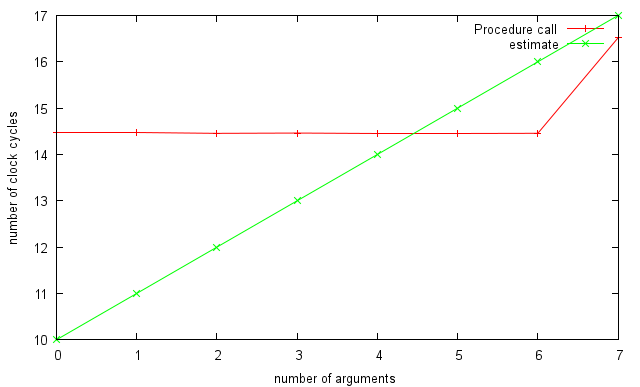
\includegraphics{procCallImage}
That's not much work and the total cost of a procedure call should be around 15
cycles. Each argument may increase the overhead of 1 of 2 cycles.
The result shows us that the base result for a procedure call is around 15
cycles and that each argument increase the cost by 1 or 2 cycles as excepted.

\subsubsection{System call overhead}
We choosed the getpid() system call to test the overhead for a minimal system
call as it's supposed the least expensive system call.
System call are excepted to be more expensive than simple procedure call as they
produce a context switch.
The result shows that a system call takes around 800 clock cycles to complete.

\subsubsection{Task creation time}
For testing the overhead of creating a new process, we simply called fork(). It turned out that it takes about 750,000 clock cycles for creating it without caching and less than 500,000 with caching.While for the overhead of creating a new thread, we simply called pthread\_creat(). It turned out that it takes about 2000,000 clock cycles for creating it without caching and less than 80,000 with caching.
The fact thread creation without caching is taking way longer time than the one for process creation doesn't really make sense to us right now, and we will look into that later as the project goes. But considering that thread creation does't envolve memory alloction, the average case for thread creation is generally faster then the one for process creation.


\subsubsection{Context switch time}
We measured the context switching overhead for both processes and threads. The way we define context switching is by creating a child process/thread and make the child do some task and return back to the parent. The overhead of such context switching is going to be the time start from the creation of the child to the time execution gets back to the parent process/thread excluding the time for child to execute. We only tested the context switching within 2 different processes.
//***TODO actual result

\subsection{Random Access Memory}

\subsubsection{RAM access time}
We measured the back-to-back-load RAM access latency, because it is well accepted by most software developers and system researchers. The way we measure the RAM access latency is making the program iterating a array of specific size for bunch of times and averaging it to eliminate the noise. The size of the array we used are larger than 256KB, which is larger than the total amount of L1 cache and L2 cache. We did multiple number of tests on iterating the first k element of the array, so that certain part of the data will be cached into L1 cache or L2 cache.
We expected to see the RAM access time increases as it goes from L1, L2 to main memory. Basically saying there would be a significant difference among the following three cases: 
1. iteration of the first 32KB data or less (fit into L1 cache)
2. iteration of the first 288KB data or less (fit into L1+L2 cache)
3. iteration of all the whole array(doesn’t fit into caches).
The result we got from our measurement shown that //TODO actual result






\subsubsection{RAM bandwidth}

We used an array with size 16MB, so that it is larger than the cache size (6MB including fancy L3 cache). At the same time, it still fits into the main memory. We iterated through the list and do both read and write. We did read by just doing a[i]+0 and write by doing a[i] = a[i]+1. We would expect read is faster than write operation, because the system need to make sure the data is actually write to the memory after performed the write operation. While there is no such issue for read operation.





\subsubsection{Page fault service time}

In order to manually create a page fault situation, we used two really large array which as the same size as main memory. Then we are going to iterate through the first array, basically means put it into main memory first. Afterwards, we iterate through the second array so that the first array will be totally paged out to hardddisk after that. The page fault service time is going to be the time it takes for us to get the value of element from first array at this point.This forces the page to swap gives us the right page fault service time. 

